% The Petersen graph: outer pentagon, inner pentagram, spokes. srg(10,3,0,1), spectrum 3, 1^5, (-2)^4.
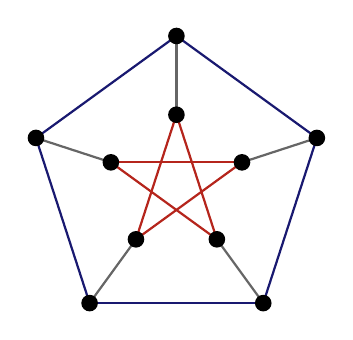
\begin{tikzpicture}[scale=1.25]
\draw[MidnightBlue,thick] (0.000,1.500) -- (-1.427,0.464);
\draw[BrickRed,thick] (0.000,0.700) -- (-0.411,-0.566);
\draw[black!60,thick] (0.000,1.500) -- (0.000,0.700);
\draw[MidnightBlue,thick] (-1.427,0.464) -- (-0.882,-1.214);
\draw[BrickRed,thick] (-0.666,0.216) -- (0.411,-0.566);
\draw[black!60,thick] (-1.427,0.464) -- (-0.666,0.216);
\draw[MidnightBlue,thick] (-0.882,-1.214) -- (0.882,-1.214);
\draw[BrickRed,thick] (-0.411,-0.566) -- (0.666,0.216);
\draw[black!60,thick] (-0.882,-1.214) -- (-0.411,-0.566);
\draw[MidnightBlue,thick] (0.882,-1.214) -- (1.427,0.464);
\draw[BrickRed,thick] (0.411,-0.566) -- (0.000,0.700);
\draw[black!60,thick] (0.882,-1.214) -- (0.411,-0.566);
\draw[MidnightBlue,thick] (1.427,0.464) -- (0.000,1.500);
\draw[BrickRed,thick] (0.666,0.216) -- (-0.666,0.216);
\draw[black!60,thick] (1.427,0.464) -- (0.666,0.216);
\fill[black] (0.000,1.500) circle (2.40pt);
\fill[black] (-1.427,0.464) circle (2.40pt);
\fill[black] (-0.882,-1.214) circle (2.40pt);
\fill[black] (0.882,-1.214) circle (2.40pt);
\fill[black] (1.427,0.464) circle (2.40pt);
\fill[black] (0.000,0.700) circle (2.40pt);
\fill[black] (-0.666,0.216) circle (2.40pt);
\fill[black] (-0.411,-0.566) circle (2.40pt);
\fill[black] (0.411,-0.566) circle (2.40pt);
\fill[black] (0.666,0.216) circle (2.40pt);
\end{tikzpicture}
